\section{Como correr o programa}

Para correr o programa desenvolvido temos várias opções. Para saber qual a sintaxe pela qual o programa se rege deve-se chamar o programa com um argumento ou sem argumentos escrevendo no terminal uma das seguintes opções:
\begin{itemize}
	\item perl test\_cmd\_wsdl.pl
	\item perl test\_cmd\_wsdl.pl -h
\end{itemize} 
\hfill\newline
\par Caso se pretenda saber quais as opções de input disponíveis para cada operação devemos inserir uma das seguintes opções:
\begin{itemize}
	\item perl test\_cmd\_wsdl.pl -o test -h
	\item perl test\_cmd\_wsdl.pl -o gc -h
	\item perl test\_cmd\_wsdl.pl -o ms -h
	\item perl test\_cmd\_wsdl.pl -o mms -h
	\item perl test\_cmd\_wsdl.pl -o otp -h
\end{itemize}
\hfill\newline
Para testar as várias operações basta inserir um dos seguintes comandos no terminal, adicionalmente pode-se escolher se se usa a opção -prod ou não com cada comando:
\begin{itemize}
	\item perl test\_cmd\_wsdl.pl -o test -f  ../LICENCE -u ''user phone number' -p 'your pin'
	\hfill\newline
	\item perl test\_cmd\_wsdl.pl -o gc -otp 'OTP received in your device' -procId 'ProcessID received in the answer of the   CCMovelSign/CCMovelMultipleSign command'
	\hfill\newline
	\item perl test\_cmd\_wsdl.pl -o ms -u 'user phone number' -p 'your pin'
	\hfill\newline
	\item perl test\_cmd\_wsdl.pl -o mms -u 'user phone number' -p 'your pin'
	\hfill\newline
	\item perl test\_cmd\_wsdl.pl -o otp -otp 'OTP received in your device' -procId 'ProcessID received in the answer of the   CCMovelSign/CCMovelMultipleSign command'
\end{itemize}
\newpage
Caso corra a aplicação com o comando \textit{test} o resultado esperado deve ser o seguinte:
\begin{figure}[H]

  \centering
  \captionsetup{justification=centering}

  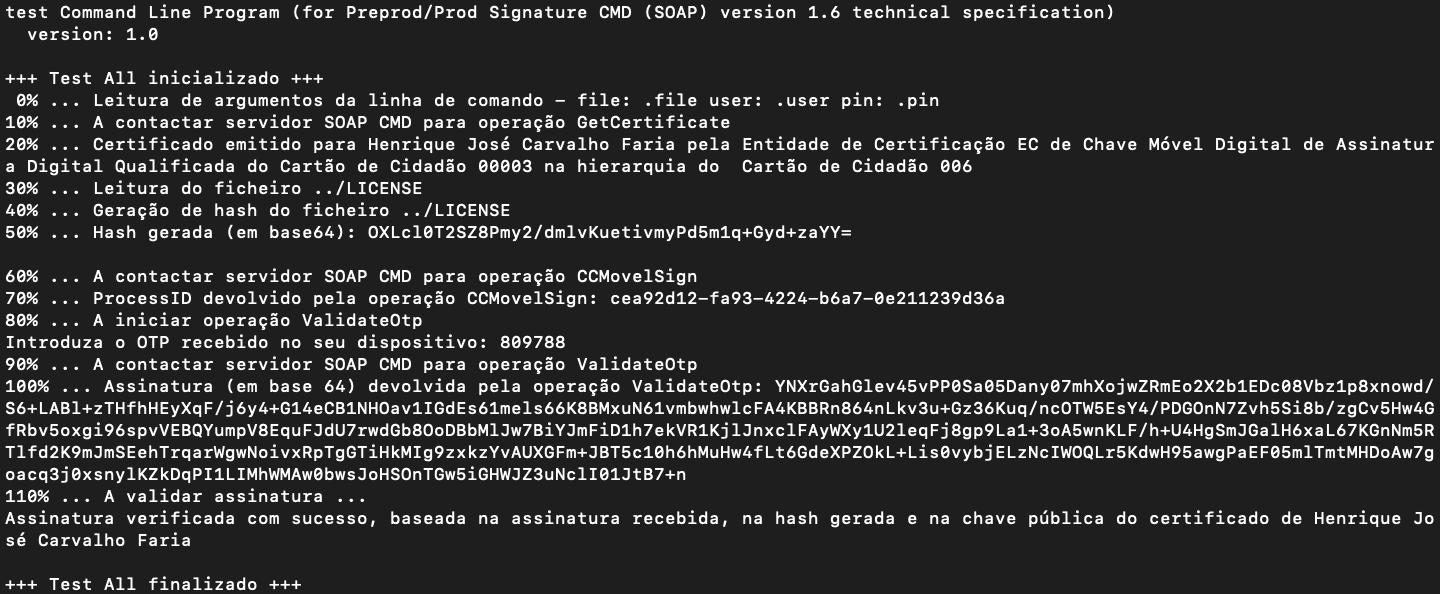
\includegraphics[scale = 0.25]{resultado.png}
  
  \caption {Resultado de correr o comando perl test\_cmd\_wsdl.pl -o test -f  'file name' -u 'user phone number' -p 'your pin' com ou sem a opção prod}

  \label {fig01}

\end{figure}